\documentclass[a4paper, 12pt]{report}
\usepackage[australian]{babel}
%\documentclass[a4paper, 12pt, openany]{book} %chose the paper size and font size. Openany ensures that all all chapters and similar may begin at any page, not only odd pages. For the introductory pages and appendices we want openany, but for chapter pages in the main content we want chapters to begin only on odd pages (right hand side). The book class ensures that the margins are automatically adjusted such that left hand pages are slightly moved to the left and vice versa at the right, which makes the thesis very readable and good looking when printed in bound book format.
\usepackage[utf8]{inputenc} %to manage special characters
\usepackage[T1]{fontenc} %to manage special characters
\usepackage[Bjarne]{fncychap} %fancy chapter style (many more available, like Sonny or Lenny etc.)
\usepackage[bf]{caption}
\usepackage{subcaption}
\usepackage{fancyhdr} %to customize the headers
\usepackage[lmargin=1in, rmargin=1in, tmargin=1in, bmargin=1in]{geometry} %sets the margins for the pages
\setcounter{tocdepth}{2} %table of contents number depth for subsections (2 = x.x.x)
\setcounter{secnumdepth}{4} %numbering depth for headers for subsections in the text(4 = x.x.x.x)
\usepackage{url} %to include urls
\usepackage{listings} %include this if you want to include code in the thesis
\usepackage{amsmath,amssymb} %mathematical package
\usepackage{siunitx} %includes SI-units
%\usepackage[bf]{caption} %makes float captions bold
\usepackage{array, booktabs} %to make better tables
\usepackage{graphicx} %to include graphics
\graphicspath{{./Figures}}
\usepackage{float} %to include floats
\usepackage[export]{adjustbox} %to adjust floats
%\usepackage{subfig} %to include subfigures
\usepackage{chngcntr} %will make it possible to change the counter for tables, figures etc. such as below
\counterwithin{figure}{chapter} %change counter for figures within sections (also possible to choose for each chapter
\counterwithin{table}{chapter} %change counter for tables within sections
\usepackage{color, xcolor} %edit e.g. text colors
\usepackage{cleveref}
\usepackage{parskip}

%\usepackage{tgtermes}

\usepackage[backend = bibtex,
            style = numeric,
            date = long,     % Long: 24th Mar. 1997 | Short: 24/03/1997
            sorting = none,
            maxcitenames = 2,   % max names to include before et. al.
            ]{biblatex} %customize the look of your citations and bibliography
\addbibresource{bibliography.bib}
%\bibliography{bibliography} %declare the bibliography resource
\usepackage{comment} %to be able to comment out sections in the .tex files
\usepackage{afterpage} %to customize page commands such as below
\pagestyle{plain}
\fancyhead[L]{Specialization Project \\ IP502122}
\fancyhead[C]{Candidate 10016}
\fancyhead[R]{\today}

\lfoot{}
\fancyfoot[C]{\thepage}
\rfoot{}



\begin{document}
%%%%%%%%%%%%%%%%%%%%%%%%%%%%%%%%%%%%%%%%%%%%%%%%%%%%%%%%
%\begin{comment}
% The title page:
% For NTNU students this page will be generated automatically when submitting your paper, and should not be included in the final file from Latex. Delete or comment out the title page setup. The final report should then start with the first page being the abstract. I have included a title page here so it is possible to see how it may look like, and for those who does not get an automatically generated title page. Of course you will need to change the names and titles etc. to your case.

%the title page should be an odd page (right hand side)

\begin{titlepage}
\newgeometry{left=2in, right=2in}
\vspace*{1.5cm}

%\noindent  \textcolor{gray}{\large Magnus Renaa Kjørseng} \\
\noindent  \textcolor{gray}{\large Candidate number 10016} \\
\vspace{1cm}

\noindent \textbf{\Large Simulation of a coupled system consisting of a non-buoyant remotely operated vehicle and a surface vessel} \\
\vspace{0.5cm}

%\noindent {\large Any undertitle is written here} \\



\vspace{7cm}
\noindent Specialization Project Report, IP502122 \\
%Supervisor: Øivind Kåre Kjerstad \\
%Co-supervisor: Co-supervisor Name \\
December 2024 \\

\vspace{0.2cm}
\noindent Norwegian University of Science and Technology \\
Faculty of Engineering \\
Department of Ocean Operations and Civil Engineering \\

\begin{figure}[h]
    
\includegraphics[width=0.28\textwidth]{ntnu_basic.png}
\end{figure}
\end{titlepage}
\restoregeometry
%\myemptypage %empty page such that the abstract starts at the first right hand side after the title page
%\end{comment}
%%%%%%%%%%%%%%%%%%%%%%%%%%%%%%%%%%%%%%%%%%%%%%%%%%%%%%%%

% The pre-chapters
\chapter*{Abstract} %pre-chapters should not be numbered, hence the "*"
%\pagenumbering{roman} %introductory pages should be roman
\setcounter{page}{1}
\addcontentsline{toc}{chapter}{\protect\numberline{}Abstract} %add the chapter to the table of contents, this is not automatically added when creating unnumbered chapters (*). Add it in a chapter style, and keep all chapters on the same numberline indent regardless of number or not on the chapter
A Remotely Operated Vehicle (ROV) can be used to find and grab underwater plastic litter. Lifting heavier litter is difficult however. This project simulates an ROV which is negatively buoyant, that is it sinks in water. The project uses Algoryx' AGX as a framework for simulating a coupled system consisting of a surface vessel and an ROV, connected by a flexible tether. 

The results of this project show that AGX is a usable framework for simulating this type of problem. Additionally the project has created a simulation which is usable for further work with this configuration of a non-buoyant ROV. Using the simulation, a simple proportional-derivative controller has been implemented and tested. 

The report concludes that the simulator created is useful in further exploration on the topic of non-buoyant ROVs. 

%Write an abstract/summary of your thesis, and state your main findings here. \\

%\noindent A summary should be included in both English and any second language, if this is applicable, regardless if the thesis is written in English or in your preferred language. These should be on separate pages, the English version first.







 %insert the chapter text from the files

%\chapter*{Preface}
%\addcontentsline{toc}{chapter}{\protect\numberline{}Preface} 
%
Write the preface of your thesis here. \\

\noindent You may include acknowledgements and thanks as part of your preface on this page, or you may add it as a new chapter after the preface.

\tableofcontents
%\addcontentsline{toc}{chapter}{\protect\numberline{}Contents}

%add to table of contents list of figures and tables, and insert list of figures and tables
%\addcontentsline{toc}{chapter}{\protect\numberline{}\listfigurename}
%\listoffigures
%\addcontentsline{toc}{chapter}{\protect\numberline{}\listtablename}
%\listoftables


\chapter*{Abbreviations}
\addcontentsline{toc}{chapter}{\protect\numberline{}Abbreviations}
% Put in your abbreviations here

\begin{itemize}
    \item \textbf{CoG} Center of Gravity
    \item \textbf{ROV} Remotely Operated Vehicle
    \item \textbf{PD} Proportional-Derivative [controller]
    \item \textbf{NTNU} Norwegian University of Science and Technology (Norsk Teknisk og Naturvitenskapelig Universitet)
    
\end{itemize}
%\newpage
%\myemptypage
%add an empty non-counted page by the command below in order to get the first chapter on the left hand side, if needed (check your page number so that the first chapter is on an odd page)


%%%%%%%%%%%%%%%%%%%%%%%%%%%%%%%%%%%%%%%%%%%%%%%%%%%%%%%%
%Customize the layout of the main content of your thesis

%\pagestyle{fancy} %set customized page style for header
\fancyhf{} %clear header and footer fields
\renewcommand{\headrulewidth}{0pt} %set to no rule
%\fancyhead[LE, RO]{\thepage} %set the page number at left for even, right for odd pages
%\fancyhead[RE, LO]{\leftmark} %set the chapter name at right for even, left for odd pages
%is is possible to design the header with the chapter as you wish, e.q. only the chapter or only the name, all lowercase instead etc.
%you could also design the footer if you wish, for example:
%\fancyfoot[LE, RO]{\thepage}
\setlength{\headheight}{14.49998pt} %set the header height


%%%%%%%%%%%%%%%%%%%%%%%%%%%%%%%%%%%%%%%%%%%%%%%%%%%%%%%%
%main content 

%\pagenumbering{arabic}
\chapter{Introduction}
\documentclass[class=article, crop=false]{standalone}
\usepackage{graphicx}
\graphicspath{{../Figures}}

\begin{document}
% The subsections written are only suggestions, to display how sections and subsections may look for your thesis

\end{document}
\section{Marine plastic pollution}
Plastic pollution in the oceans has been widely documented, however the amount of plastic currently in the ocean is uncertain. Jambeck et al.\cite{jambeck_plastic_2015} estimates that in 2010, somewhere between 4.8 and 12.7 million metric tons(MT) of plastic ended up in the ocean. According to the World Economic Forum\cite{world_economic_forum_top_2022}, there is between 75 and 199 million MT of plastic waste currently in the ocean. Around two thirds of all plastics that end up in the ocean are heavier than seawater \cite{isobe_fate_2022} meaning that they sink and either drift in the pelagic zone or end up on the seafloor as litter. Removing litter and plastic pollution on a large scale is difficult, removing it under many meters of ocean makes it much more difficult. 

It is undesirable to have plastic waste in the oceans. This is because of the health effects the plastics have on marine and terrestrial life. Two points are especially of note: microplastics and leeching. Microplastics are plastic particles smaller than 5mm. Leeching on the other hand, is the plastics' chemical interaction with the seawater surrounding them, leeching harmful chemicals into the water.\cite{prata_environmental_2020}\cite{zolotova_harmful_2022}\cite{segovia-mendoza_how_2020}\cite{obuzor_chemical_2023} For both of these issues, the best solution is to remove the litter. This is because plastics' general longevity. For example, Oluwoye et al. \cite{oluwoye_degradation_2023} found that polyethylene, commonly used as a coating for subsea structures, would take about 800 years to degrade on the ocean floor. Polyethylene is also used in many consumer- and industrially facing applications, for instance in plastic cannisters for liquids, boxes and crates for fishing or other industrial practices, or as plastic bags. 

\section{The Plan Sea Project}
The desire to deal with sub-surface marine plastic waste, i.e. litter both in the pelagic zone and on the seabed, was what sparked the Plan Sea project. Plan Sea is a student driven project at NTNU in Ålesund with the goal of finding, developing and testing a potential solution for removing sub-surface plastics. The project is at time of writing still in its early phases and ongoing. At time of writing, a hull has been constructed from carbon fiber sandwich boards. Thrusters have been mounted to the hull and work on controlling them has started. Additionally, an ROV has been acquired for the project. 

Since this is not a report focused on the Plan Sea project, the proposed solution arrived at in Plan Sea will not be discussed in detail. However, because of the relationship between this project and Plan Sea, it is necessary to describe the solution at a surface level. 

\subsection{The proposed solution}
The solution which the Plan Sea project is aiming for is an ROV-based solution with an unmanned tender-vessel on the surface. The ROV has a gripper attached and will navigate to find litter, grab it and pick it up. The surface vessel exists to provide the ROV with a greater lifting capacity. If the ROV was to lift purely under the force of its own thrusters, as is traditional for ROVs, the total amount of lifting force available would be limited by the vertical thrust available. This would mean that either the ROV would have to have a very large amount of vertical thrust available relative to its size, or that the total lifting capacity would be very small, neither of which are desirable. By connecting the ROV to the surface vessel with a winch and a lifting cable, it is possible to use the ROV to do fine-navigation to find and attach to litter, and then use the lifting force of a winch and the total buoyancy of the surface vessel for lifting heavier objects. Ideally an ROV which originally only has a total lifting force of about 15kg would be able to lift heavy cables or car tires. Additionally, the solution is supposed to have an undersea basket for collection to avoid having to lower the ROV to the seabed and then lift it up to the surface for each piece of waste. Instead the ROV can be lowered down and can pick litter it finds and place it in the basket. Once the basket is full it can then be lifted up and either emptied on deck, exchanged for another basket or taken back to shore for further sorting there. A sketch of the solution can be seen in \cref{fig:overview}.

\begin{figure}
	\centering
	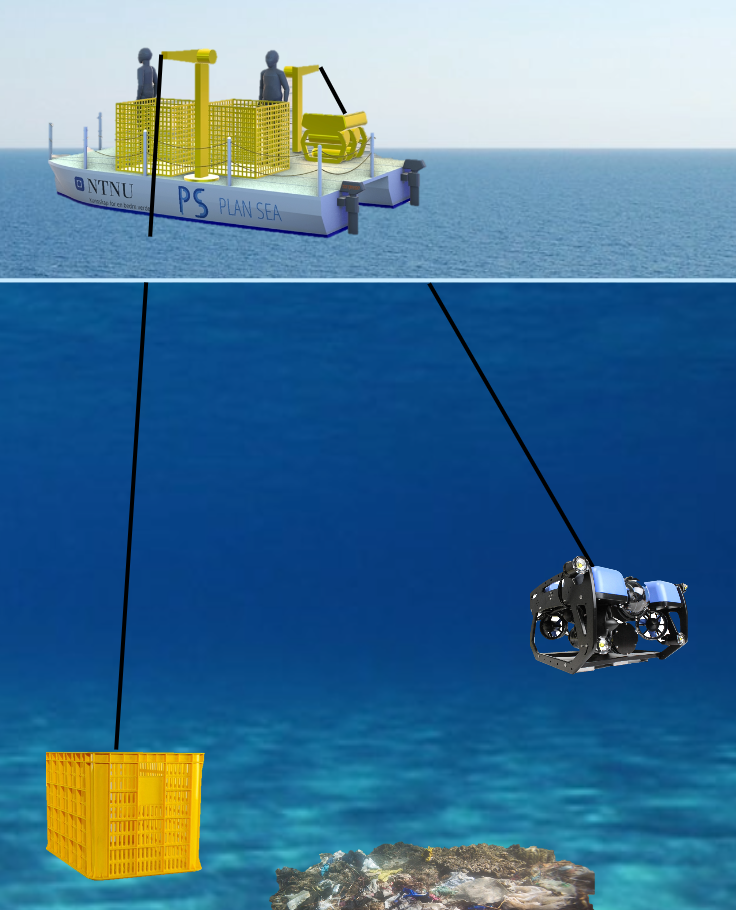
\includegraphics[width=0.5\textwidth]{overview}
	\caption{A sketch of the proposed solution for Plan Sea showing a surface vessel, a tethered ROV and a collection basket}
	\label{fig:overview}
\end{figure}

Using this solution allows for completely ignoring the buoyancy of the ROV, unlike traditional ROVs. Traditional ROVs are generally designed to be neutrally buoyant, meaning that they neither sink nor float, but keep their vertical position in water once placed there. Since the Plan Sea ROV will be attached to a cable to the surface vessel at all times, it can instead hang from the cable. This means that it's possible to attach larger grippers, more battery capacity, more detection/lighting/navigation equipment, and otherwise allows for any desired modifications to be done to the ROV. Additionally, since the ROV doesn't need to provide vertical thrust, it is much easier to not disturb the seabed which will provide a clearer view for detection equipment based on visible or near-visible light. However, having a non-buoyant ROV does come with some drawbacks.

One drawback of this solution is that it will switch between two operating modes, searching/grabbing and lifting. In the search/grab mode the ROV will be near-neutrally buoyant, or somewhat negative. When lifting the ROV might be severely negatively buoyant. These two wildly different operating modes increase the needed complexity of the system. Another drawback is that as the ROV is hanging from the cable, it creates a coupled system consisting of the surface vessel and the ROV, and necessitates the two moving together as one unit. The forces the surface vessel experiences, such as waves or wind, will impact the ROV, likewise currents or snags the ROV experiences will affect the surface vessel.

\section{Control systems}
A control system commands and regulates the behaviour of other systems automatically. For this project in particular, the control system will be in charge of maintaining and changing positions of the two vessels. A simplified function block diagram of the total system can be seen in \cref{fig:fbd}. The goal of the simulator is to function as a drop-in replacement for the vessel, local controllers and environmental impact shown in the figure. This makes it so that the development can happen digitally to then be quickly deployed in the real-world.

\begin{figure}
	\centering
	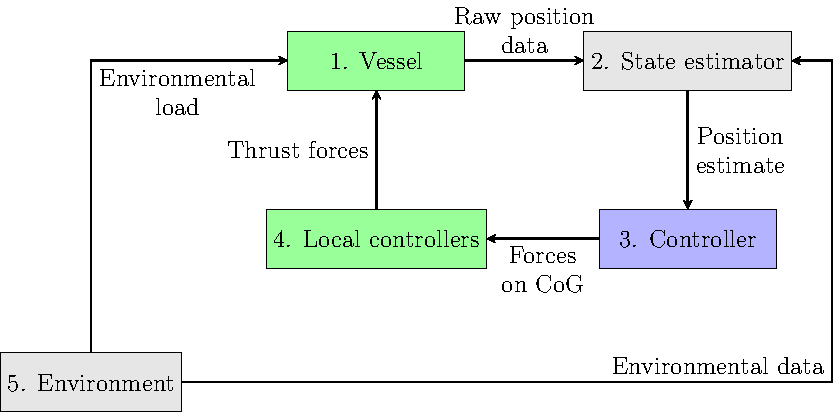
\includegraphics[width=0.8\textwidth]{control-fbd}
	\caption{A simplified function block diagram of the total system. Grey blocks are not currently implemented, green blocks are simulated and blue is for the controller which is system-agnostic}
	\label{fig:fbd}
\end{figure}


\subsection{Considerations because of a coupled system}
In the marine sector, dynamic positioning (DP) is commonly used. DP allows for a vessel to maintain a position or a course automatically despite external effects. This is used for example for offshore supply vessels which need to stay stationary relative to an anchored platform to allow loading and offloading of supplies. DP is also used for applications such as laying subsea fiberoptic cables, where maintaining correct speed and course is important to avoid damaging the cables. For the Plan Sea project too, a DP system is necessary because it consists of vessels that need to maintain specific positions at sea with wind, wave and current forces affecting the vessels

Normally a DP system only considers one vessel, however for the Plan Sea project it has to be more comprehensive than that because the two vessels are coupled. This is all further discussed in \cref{sec:math}

\subsection{The need for rapid prototyping}
Rapid prototyping is becoming increasingly popular with time. The goal of rapid prototyping is to create some simulated environment in which you can test and iterate on a solution until it is acceptable. Then, once you have a solution that works within a certain level of acceptability you can start to put materials and resources into building and implementing the solution in the real world. 

For my purposes, rapid prototyping will allow me to experiment with control system tuning and variables without having to deploy the full-scale vessel every time. Ideally, the solution arrived at in the prototyping stage will be directly applicable to the full-scale version, which allows for rapid deployment. The hope is that any issues will be detected and solved while testing digitally, meaning that we hopefully avoid large surprises during deployment. 

\section{Problem description}
A simplified sketch from \cref{fig:overview} can be seen in \cref{fig:simple}. It shows the three main components of this system: The surface vessel, the ROV, and the tether between them. It also shows the forces in the tether. As the tether holds the ROV up, the tether pulls the surface vessel down. This follows from Newton's second law of motion. The figure also shows the coupled nature of the system, since the tether will be taut at all times, both vessels will experience this force from the other at all times.

\begin{figure}
	\centering
	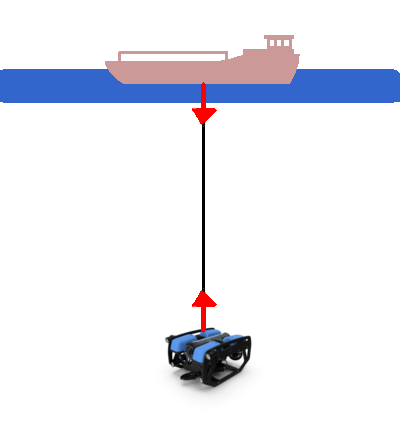
\includegraphics[width=0.6\textwidth]{simplified-overview}
	\caption{A simplified sketch of the problem, forces experienced by each vessel are shown in red. Forces are not to scale.}
	\label{fig:simple}
\end{figure}

In \cref{fig:angled} two scenarios are shown overlaid, one where the ROV is hanging straight below the surface vessel and another where it is at an angle. The result is that the ROV is not at a constant height. If we imagine a desired elevation above the seafloor is constant, then either the ROV needs to have more tether payed out and provide lift through its own thrusters, or the surface vessel needs to move to allow the ROV to hang perpendicular to the surface of the sea. If more tether was to be payed out and the system then stabilizes, the ROV will fall to the lowest possible point. It is possible then that the ROV might collide with the seabed or other objects. The ideal solution then becomes that the surface vessel follows the ROV, or the ROV only operates within a given area of operations directly underneath of the surface vessel. 

\begin{figure}
	\centering
	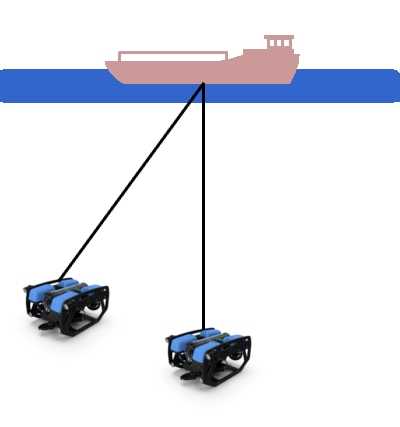
\includegraphics[width=0.6\textwidth]{angled}
	\caption{The ROV is hanging from the same point on the surface vessel with an equal tether. Note how the height of the ROV has changed because the tether has stayed the same}
	\label{fig:angled}
\end{figure}

Further, this non-perpendicular arrangement will lead to tangential forces, shown in \cref{fig:angled-force}. The forces will of course be equal and opposite on the vessel's end, though this has been omitted from the figure for clarity. The horizontal force the tether imparts on the ROV will act as a restoring force, trying to move it back to be perpendicular to the surface vessel. The surface vessel likewise will experience a pull towards the ROV. 

\begin{figure}
	\centering
	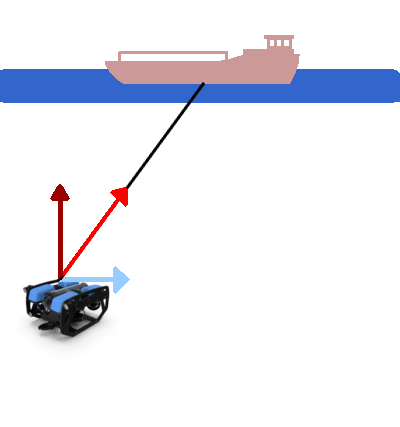
\includegraphics[width=0.6\textwidth]{angled-component}
	\caption{The component forces on the ROV resulting from an angled lift, decomposed}
	\label{fig:angled-force}
\end{figure}

Because these two vessels are connected, and therefore dependent on each other's positions, the control system needs to take this into account. Probably, the simplest solution will be to have one large control system handling both, or alternately having one of the vessels take a leading part and the other attempt to follow. This will be touched on later in this report, though not discussed in detail.

\section{Statement of intent}
For this project I want to create a simulation which is able to quantify the effects that the parts of the system have on each other. I want to be able to measure the tension in the wire, the force exerted by the vessels, how well the vessels follow each other or orders given and influence from the environment. The goal of this simulation is to be used as a future design tool for finalizing design of the Plan Sea vessel, its control systems, as well as defining operational criteria. 
\end{document}
%\cleardoublepage
%the cleardoublepage command ensures that the next text page is on the right-hand side (odd page) and produces a blank page if necessary to achieve that, as all chapters should begin on the right hand side


\chapter{Modelling and Control Design}
\documentclass[class=article, crop=false, draft=true]{standalone}
\usepackage{graphicx}
\graphicspath{{../Figures}}

\usepackage{amsmath}

\usepackage{cleveref}

\begin{document}
%equations, bib. \\
\section{Previous project work}

\section{State of the Art}
\subsection{Physical issues}
\subsection{Simulation issues}

\section{Mathematical basis}


\section{Modelling and Control Design}

\begin{figure}
    \centering
    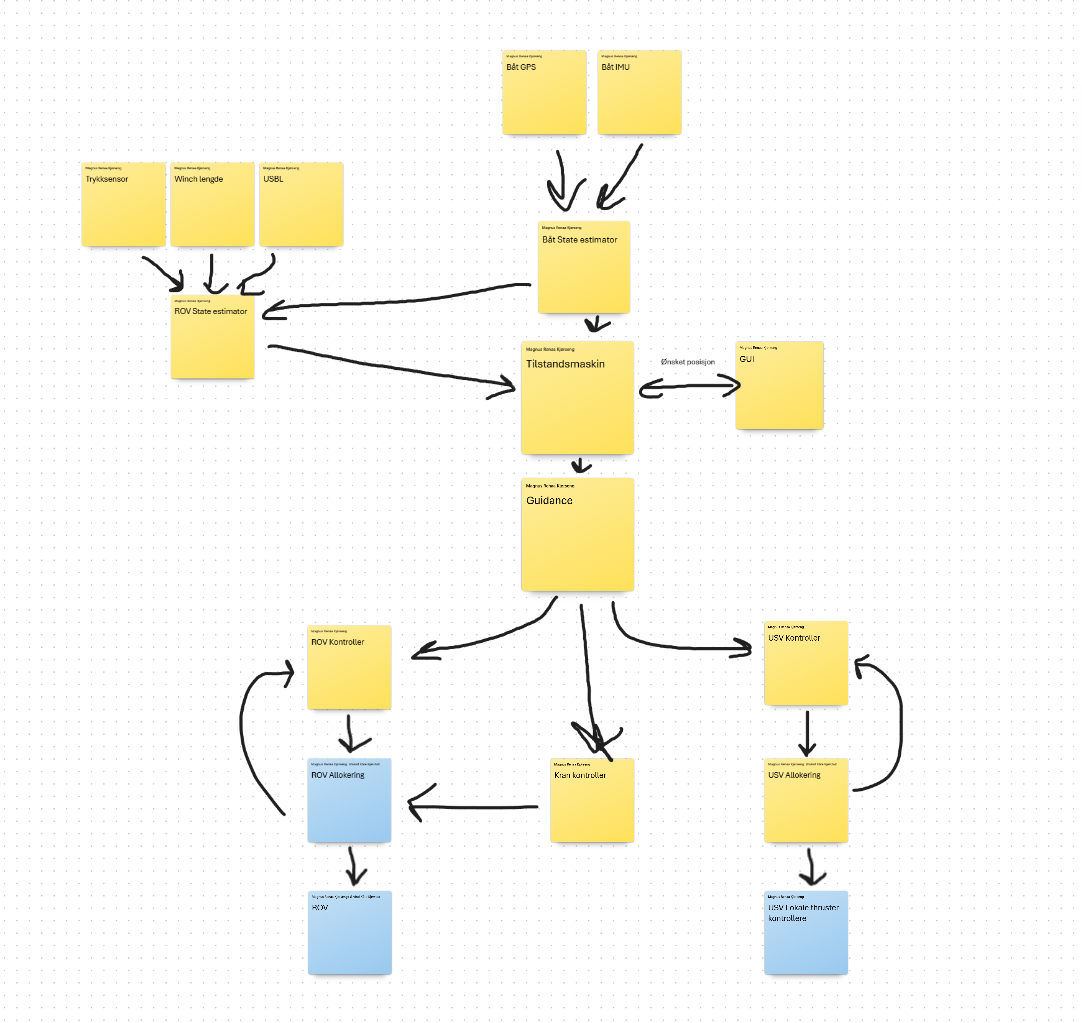
\includegraphics[width=0.9\textwidth]{control-system}
    \caption{A sketch of the control system design. TODO: Fiks bedre illustrasjon}
    \label{fig:control-system}
\end{figure}

\section{Sensorics}
The first step to knowing where to go is knowing where you are.

There are several pieces of sensorics that will be used for positioning of the system.

\subsection{GNSS}
Firstly, Global Navigational Satellite Systems, or GNSS, will be used to position the USV. There are several separate systems for GNSS, including GPS, Gallileo and GLONASS to mention a few.

The exact workings of how GNSS works is not essential for this project. The important part is that GNSS requires a clear view of the sky and allows for accuracies of approximately 2m. While this accuracy would be usable for this project, a higher accuracy would be preferable. Luckily, there exist systems that allow for this greater accuracy as well. For this project, an RTK enabled GNSS reciever has been acquired. RTK uses a secondary base station and direcct communication between the receiver and the base station to produce highly accurate readings, on the order of millimeters or centimeters, as opposed to meters.

GNSS requires a clear view of the sky, this means that it's not usable indoors to a large extent, and it's also not usable under water. Water is an excellent absorber of the entire spectrum of electromagnetic radiation, from radio all the way to gamma rays. This means that separate positioning is required for positioning the ROV.

NMEA-0183 GGA message used for recieving position

\subsection{USBL}
The main method for positioning the ROV will be through an ultra-short baseline system, USBL. USBL works sonically by having a tranciever on the surface vessel which transmits a sound signal, the signal is picked up by a transponder under water which transmits a response signal. The tranciever through an array of hydrophones picks up the response and is able to find the direction it came from as well as the distance. Direction comes from differential time of response for the different hydrophones, while distance comes from a combination of time-of-flight and doppler (TODO: sjekk om doppler faktisk er en greie her).

TODO: Legg inn figur av USBL

Available and accurate

Need to consider limitations of accuracy of USBL re: salinity, water temperature/density, etc.

\subsection{IMUs}
Both the surface vessel and the ROV will have inertial monitoring units, IMUs, installed. These detect changes in velocity and acceleration in 6dof, allowing for relative position to be found. IMUs are most useful as a dead-reckoning tool, i.e. using a last known location and a set of velocities/directions, an approximate current position can be found.

For this solution, the IMUs will be used as supplemental data to the USBL and GNSS systems. This is to allow for a more complete model of the movement of each of the vessels. Especially for the surface vessel, things like heave from waves is not necessarily easy to get from GNSS data, but will be trivial to find from an IMU. Using this it's also possible to potentially build a model of the current seastate which allows for better predictive DP rather than just a reactive system which is what's currently implemented.

\subsection{ROV Depth measuring devices}
The ROV will have a couple of extra sensors for finding depth and distance from the seafloor.

A pressure sensor is able to fairly accurately (within 1m) tell the depth of the ROV. Pressure sensors can work in many ways, the ones available here use a two chamber differential approach with a flexible membrane between two chambers. One chamber is open to the atmosphere and the other is closed off with a known pressure inside. By measuring the amount the flexible membrane stretches, it is possible to find the pressure differential between the two chambers. Knowing this differential and the calibration pressure, it's possible to estimate the depth by using the knowledge that water pressure increases by approximately 10kPa per meter of depth. More accurate values can be found but depend on things like water temperature, salinity and others.

Another tool which will give an upper bound to the depth of the ROV is the length of wire which has been payed out. Due to effects because of lag and currents as mentioned previously (TODO: faktisk skrive dette) the length of the wire will in most cases be greater than the actual depth of the ROV or the distance to the ROV. It can still be useful to know this length though, both as an absolute upper bound to fact-check the other sensors, but also to keep track of how much of the wire remains and how the winding system may work.

Additionally, the ROV will be mounted with a laser based time-of-flight sensor. This sensor works similarly to the USBL system mentioned above but using laser light instead of sound. A laser is sent from the sensor, hits obstacles or the seafloor and bounces back. The light bouncing back is detected by the sensor and doing time-of-flight calculations, it's possible to find the distance from the sensor to the object in question. This can be done to very accurately measure the distance to objects or the seafloor to avoid collisions or aid in picking them up.

Another example of something that could potentially help is taut wire positioning. Taut wire positioning works by having a wire anchored at a given point and then measuring the angle at which the wire exits a boom or whatever is holding it in place. By knowing the length of wire, the fact that the wire is taut, and the angle at which the wire is extending from the surface vessel, it is possible to find a relative position between the surface vessel and the anchor. It is possible that with a very heavy ROV, or if the ROV picks up a large load, that taut-wire might work for positioning, but given the effects on the wire seen in simulation it's very probable that taut-wire will provide more trash data than useful. Due to this it's disregarded as an option.


\section{State estimation}
The state estimator takes in the various sensor data and builds a single model of position. This is done because different sensors might have different accuracies or update times. The state estimator handles these discrepancies and builds a cohesive model. The state estimator feeds this more accurate position into the guidance system (TODO: Spørre øivind om det er guidance eller state machine som får posijonen. State machine skal jo bare være et informasjonslager?)

\section{State machine}
The state machine keeps track of variables for the total control system. These include current position, but also things like desired position or operating mode, gathered from the GUI.

\section{GUI}
The GUI is where a human operator interfaces with the control system. The GUI is supposed to include a position input for the surface vessel, mode switching between USV-Master, ROV-Master and idle/standby modes, along with other functions.

\section{Guidance}
The guidance system provides finer control of the vessel than what would be achieved by a state machine and controller alone. For instance it smooths acceleration/deceleration of the vessels by providing imaginary set points between the current position and the actual set point.

\section{Controller}
The controller finds a desired force input based on the difference (error) between the current position and the desired position. The current implementation uses a simple PID for this. This force input is fed forward to the allocator.

The shape of the force coming out of the controller is as \[\tau = \begin{bmatrix}X \\ Y \\ N\end{bmatrix}\]

\section{Allocation}
The allocator works like a translation layer between the controller and the local controllers. The controller provides a force input on the vessel's center of gravity. By inputting forces on the center of gravity, no torques are produced from lateral forces, nor lateral forces from the torque.

In abstract terms, the allocator finds and applies a transformation matrix \(T\) such that \[Tf = \tau\] where \(f\) is a vector of vectors with the lateral forces for each thruster. For this case with two thrusters, it will look something like \[f = \begin{bmatrix}x_1 \\ y_1 \\ x_2 \\ y_2 \end{bmatrix}\]
The transformation matrix can be written explicitly for the USV, since it has a very simple thrust configuration. For larger configurations it might be better to write each thruster's transformation individually and either add or remove them depending on the type of move necessary (larger moves use only larger thrusters etc.).
\begin{equation}\label{eq:transform_matrix}
T = \begin{bmatrix}1 & 0 & 1 & 0 \\ 0 & 1 & 0 & 1 \\ -l_{y_1} & l_{x_1} & -l_{y_2} & l_{x_2}\end{bmatrix}
\end{equation}

\begin{figure}
    \centering
    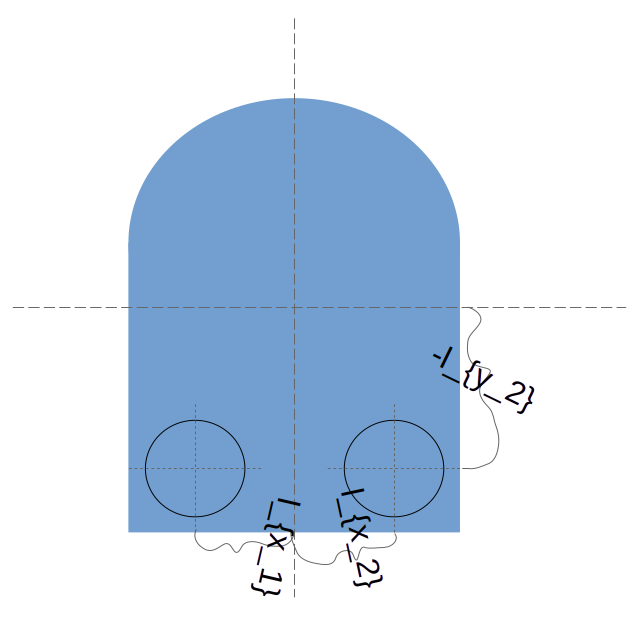
\includegraphics[width=0.9\textwidth]{thruster_position_sketch}
    \caption{Sketch of how the thruster position values in \cref{eq:transform_matrix} are found. The thruster configuration will be input to the allocator through a config file.}
    \label{fig:thruster_position_sketch}
\end{figure}

Since \(\tau\) and \(T\) are known, we can find \(f\) by performing a pseudoinverse on \(T\) leading us to the equation

\begin{equation}\label{eq:final_allocator}
f = T^\dagger \tau
\end{equation}

where \(T^\dagger\) is the pseudoinverse of \(T\).

This can also be written longform as

\begin{equation}\label{eq:long_allocator}
\begin{bmatrix}x_1 \\ y_1 \\ x_2 \\ y_2 \end{bmatrix} = T^\dagger \begin{bmatrix}X \\ Y \\ N\end{bmatrix}
\end{equation}

The full matrix for \(T^\dagger\) is omitted because the pseudoinverse of a non-square matrix tends to be large and ugly. It will only be handled by machine hands anyway, and as such doesn't matter right now.

The ROV has a built-in allocator which works well enough. The only issue with the ROV's allocator is that it's configured for a neutrally buoyant vessel. For this system we need to filter the vertical force component so the ROV only handles high-frequent/small-amplitude responses and the crane handles larger amplitudes and lower frequencies. This is also necessary because of elasticity in the lifting cable.

\section{Local control and physical response}
The vessel in this iteration has two thrusters. The ROV has a closed working solution and will not be considered here except for in the hypothetical. Each of these local controllers receive a two-component vector (or three-component in the case of the ROV) which instructs the controller what the desired thrust is. The azimuth thrusters on the USV are able to apply a force in one direction (parallel to the propeller axis), but they are able to vector this one-dimensional thrust using the azimuth ring.

\end{document}

%\cleardoublepage

\chapter{Simulation Framework}
The goal of this specialization project is to build a simulator which is applicable to the case of the Plan Sea project. There are five elements that need to be simulated for this to be considered a success. 
\begin{itemize}
\item Surface vessel
\item Subsurface vessel
\item Connecting wire
\item Weather impacts
\item Control system
\end{itemize}

Of these points, all of them can be simulated fairly simply with purely  analytical methods except for the connecting tether. Wire physics are a notoriously difficult thing to simulate because they are not rigid bodies. They have strength in tension but not in compression, leading to a discontinuous behaviour. You can't push a rope, or wire in this case. 

There are two main paths to take with regards to making the simulation. I could make everything from scratch from first principles or I could use an already existing simulation framework and build something on top of that. Both solutions have positives and negatives. 

Creating a system from scratch would be an interesting challenge. It would also give me exactly the results I'd want with very little overhead, assuming that my own programming skills are up to the task. The bespoke, home-made simulator also wouldn't have any associated licensing costs. On the other hand, to create a simulator which includes buoyancy, fluid dynamics, wire physics, handles a coupled system and also has some form of graphical interface/readout for the user is a large task to undertake. 

Using a commercially available system also has a fair few benefits. I would have a mostly ready-made framework which I can just configure the simulation at hand within. Changing out parameters and variables would also be very simple, as it's essentially the same as the original configuration. I believe also that the results from a commercial solution would be more reliable than my own attempt. It is reasonable to assume that an industrially used simulation solution made by a team of physicists, computer engineers and other specialists is fairly accurate with regards to its results. The same cannot be said for a cobbled-together solution made by one student in roughly 6 months. Commercially available solutions are not all perfect however. There are licensing costs associated with many simulation frameworks. Some having enormous costs for the scale of a student project. There is also likely more overhead with a commercially available solution due to them being as wide in their application as possible, to allow for as many customer types as possible. This can make the commercially available solution slower or less responsive. 

After considering the points above for both commercially available and personally crafted simulation frameworks, I decided that using a ready-made solution would be better. This was especially decided because of the time constraints of this project. My goal is to have a working simulation that can be used to provide information, the goal is not to make a simulator. If I was to make it myself, the project would quickly turn into "make a simulator" rather than "make a simulation", simply because of the scale of the undertaking. 

\section{AGX}
After considering multiple simulation options and on the advice of a professor, I landed on using AGX, made by Algoryx, as a simulation framework. AGX has a solid wire simulation package, a hydrodynamic simulation package, and allows for scripting and setup using both Python and C++. It has interfaces towards both Unreal Engine and the Unity engine for further graphical display of the results. In addition, AGX has interfaces for ROS2 which I will get into in \cref{sec:ros}. 

My implementation of AGX is based on Python as that's the language I'm most familiar with. I am aware of Python's inferiority to a C++ based approach in terms of speed and efficiency in resource use, but the time investment required for me to get to an acceptable level of C++ proficiency was not worth it for this project.



\subsection{Limitations of AGX}
By using a ready-made simulation platform I am able to quickly implement a simulation without needing to worry about the mathematical models that exist behind the simulation. This allows me to focus on achieving results, although it also necessitates a degree of trust in the simulation. I am able to verify whether the simulator acts as expected or not, but changing the governing equations is not necessarily something I am able to do. 

Another limitation of AGX is that it's a licensed software. This means that in order to apply and use the findings of this report, the software needs to be acquired. This is a limitation for further research, and ideally the findings should be based on open and available software or arrived at from first principles. 

\section{Description of the simulation setup}
The simulation starts with defining a water volume. This is done using AGX built-in functions. Currently the volume is 100m along the sides and 50m deep, though this is arbitrary. I've implemented one "water controller" which is the object that handles wave, current and wind forces. Currently this controller is completely still and there is no force inputs, but it is implemented so that adding weather forces is simple for later iterations. In AGX, each element in a simulation has to be individually added to that simulation. Once both the water volume and the water controller have been added to the active simulation, the vessels are made.

The surface vessel and the ROV are both implemented as children of a parent class for general vessels. I've done this for ease of expansion later. The ROV is just a simple box with a given density and size, while the surface vessel's shape is defined by an .obj file I've made that approximates the shape of the hull intended to be used for the Plan Sea project. The hull file is read by the script, and a wireframe is built based on it. If a more accurate shape for the ROV is desired, it is possible to implement it similarly to the surface vessel, but since this project is mostly a first-order approximation of the problem, I believe a simple box is sufficient.  

In addition to a class which handles the shape and properties of the surface vessel, I have made a class that handles controlling the surface vessel for now. The controller is just a simple implementation of a PID controller and is not properly tuned yet. The controller checks the position of the vessel on each timestep and calculates an error. The error is then controlled using the PID controller and a response is found. The response is clamped within a given authority limit. I've done this because realistically, the control authority of the system is going to be limited because of the physical capabilities of the thursters. I've estimated the authority for right now, but it should be changed later when the real command authority is found. 

Currently, the way the controller is acting on the vessel is by simply applying a force in a given direction on the CoG of the vessel. For the surface vessel, any force given in Z-direction is ignored as the surface vessel will not be able to cancel its own heave in waves. There is no controller yet implemented for the ROV. In the current implementation, torque/yaw is also ignored, and the vessel has no controlled heading. In a future iteration, both the simplistic control and heading control could be implemented by splitting the force inputs from one single input at CoG to one input at the position of each thruster. Then yawing motion will also be applied with differential thrust and a yaw-term can be added to the controller. 

Whether the complications mentioned in the previous paragraph are necessary is not clear yet. If we consider the ideal future implementation in a physical vessel, the controller designed now is only intended to give the total commands to the vessel. Thrust allocation and local control will be designed elsewhere and simply be a node in the ROS2 system that will be the final vessel. Either way, the option of making the simulation more true to life exists if it should be desirable. 

Finally, the wire which connects the ROV and the surface vessel is created. AGX has two similar wire-like simulation objects: Wires and Cables. According to the documentation, because torsion of the wire is irrelevant, we want to be able to winch the wire in and out to simulate lifting and lowering the ROV and we are working on long wires, the Wire module should be used. The way wires work in AGX is as a series of links connected to or passed through a series of nodes. For this implementation only two nodes are necessary, one connecting the wire to the surface vessel and one connecting it to the ROV. The Wire module of AGX allows for winches to be simulated as well, with given speeds, gearings, torques etc.. I have not implemented this currently due to time constraints. 

In addition to all the "necessary" elements, the simulation also has a manual controller for the vessels. It is possible to use the keyboard to give manual force inputs on the vessels. This uses the same framework for adding force as the controller does. I've done this as a way to debug and test the system a bit.



\section{ROS2}
\label{sec:ros}
ROS2, short for Robot Operating System 2, is an easily expandable and configurable operating system used primarily for hobbyists and research in control and robotics. The main selling point of ROS2 is its node model where different parts of a control system can be placed in separate, segregated nodes with certain interfaces. Those nodes then either publish data to or subscribe to data from what ROS2 calls topics. This system grants a developer or team of developers flexibility with regards to changing out certain nodes while still allowing the larger system to work. I.e. experimenting and changing out single nodes, so long as the same topics are still used, is extremely simple. 

I was not able to implement ROS2 during this project. I believe this is because ROS2 is not designed to be used on Windows and requires a lot of workarounds which I was not able to figure out. This section is in the report more as a reference and a reminder for future iterations based on this report that ROS2 would make the project easily scalable and iterable. 

AGX has the ability to work with ROS2, having built in methods for both publishing and subscribing to topics. Applied to this project it would in theory allow for the control system to be built in ROS2 and connected to the simulator. The control system could then be tested and tuned in different simulated environments until satisfactory results are achieved. When the control system works as intended, it can then be disconnected from the simulator and connected to a physical implementation of the simulated environment which would allow for real-world testing. 

The end result of the process above would be two equivalent systems, one digital and one physical, which would allow for rapid prototyping in the digital space before quick deployment in physical space. 


%\cleardoublepage


\chapter{Results}
\section{Simulation setup}
The finalized simulation setup consists as described in \cref{sec:setup} of two vessels connected by a tether. The vessels exist in a \(200m\times 200m\times 100m\) large water volume. The submerged vessel is denser than the surrounding water and the floating vessel is less dense. For the testing I've done I have set the tether length, and therefore ROV depth, to be 20m. This was done arbitrarily, but chosen because it allows for the effects of the system to propogate quickly, meaning stabilization time is lower. The two vessels are connected by a tether which is 10cm in diameter. This diameter was chosen mostly so it would be visible in the readout as otherwise it would be so thin as to disappear. Of course, choosing a larger tether makes the tether's impact on the results larger. This may be a source of error in the later results. The wire is defined with a Young's modulus of \(10^9\), this value was chosen as an estimate based on other somewhat similar tethers I found commercially available. 

The simulation works as would be intuitively expected. An example of the simulation graphical interface can be seen in \cref{fig:sim-display}. The figure shows a surface vessel and the ROV under water in green, and the teal tether connecting them. The simulated water is shown as a grey volume, but it's not easy to distinguish it in \cref{fig:sim-display} because it takes up the entire screen. When interacting with the interface the water volume becomes more obvious. 

\begin{figure}
	\centering
	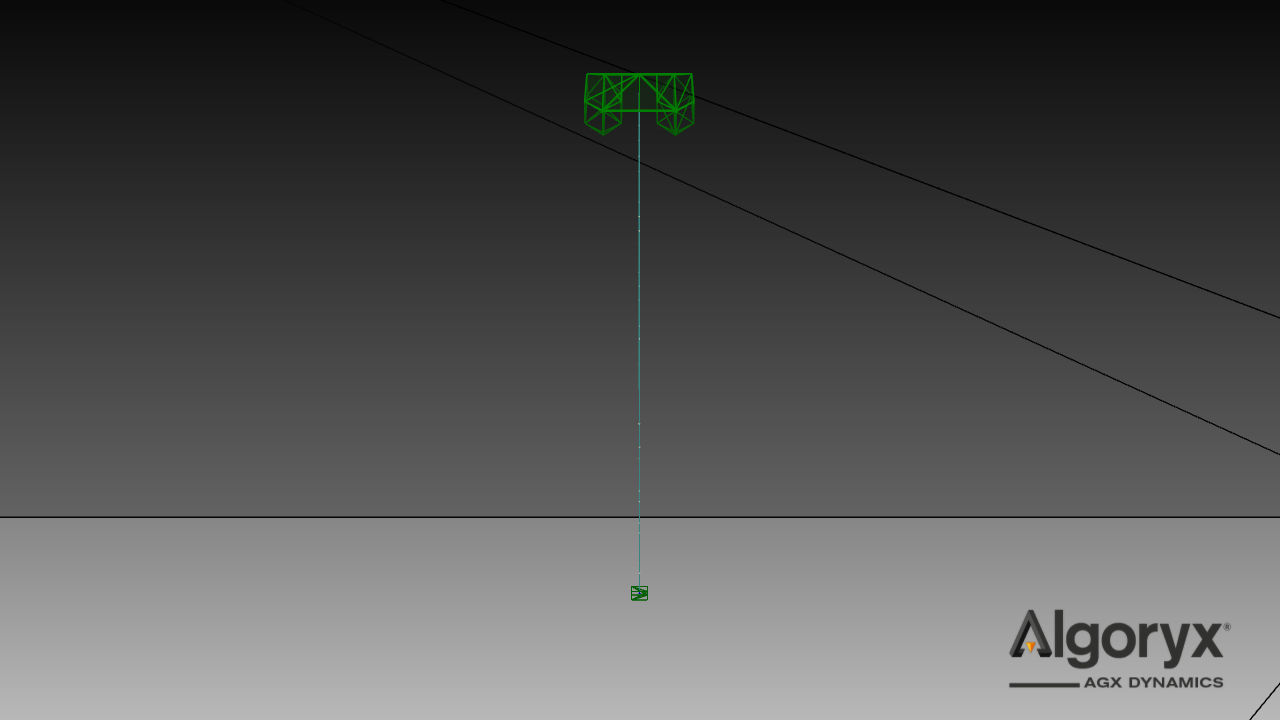
\includegraphics[width=0.8\textwidth]{sim-display}
	\caption{The graphical user interface of AGX with the simulation running}
	\label{fig:sim-display}
\end{figure}

\section{Model Validation}
\label{sec:validation}
There are two ways I will attempt to validate the simulator results here. One is intuitively and the other is using analytical methods and a simple case. The intuitive demonstration is difficult to convey in text-form in a report, but I have placed some animations of the results on GitHub\cite{noauthor_fordypogmastersimulator_nodate} alongside the simulator. The intuitive demonstrations consist of starting the simulation, pulling objects around and seeing if they "act right". Human minds are excellent pattern recognition machines, and I will use this to my advantage here, as if something is "off", it would be noticable. 

For the analytical validation I will use analytical methods and simple physics to estimate an expected result, and then simulate the result to compare the values for both.

\subsection{Intuitive validation}
I have done two tests here, one where I pull the surface vessel and look at how the ROV follows, and the other where I pull the ROV and see how the surface vessel follows. The shape of the tether is also relevant here. Looking at the results, shown in the \texttt{Results} directory of the simulator on the Github repo, there is nothing that pops out as obviously wrong. Of note is that the surface vessel flips in the ROV pulled test. This is because I pulled the ROV down and given the situation the surface vessel was in it was more stable flipped upside down. This is not a realistic scenario for the real-life project because the amount of force exerted pulling the surface vessel down will never be that large. Looking at the tension in the tether at the ROV it reaches upwards of 20kN at points, which corresponds to roughly 20 tonnes lifted.

In addition to the two tests above I've also tried swinging the ROV as a pendulum underneath the surface vessel. This test also confirms the intuitive assumption that when the surface vessel is far more massive than the ROV, it will be less affected when pulled like this, although it will still be affected. 

I will note that in the two first animations the ROV is shown as larger than in the last. This was due to an implementation error on my part. The result of this is that the ROV is far more massive than it's supposed to be, and also larger which gives it greater drag in the water. Neither of these affect the intuitive approach as the physics still "act right". 

\subsection{Analytical validation}
\label{sec:anal}
For the analytical part of the validation I will use a simple case in which the surface vessel moves forward, towing the ROV behind it. This will be roughly analogous to how the ROV and tether will respond in currents, though not entirely interchangable. The current speed will impart parallel forces on the tether and ROV while the towing case will impart a tension force on the tether. Still, this is a simple case for rough validation of the model and can be further worked or reworked for later use.

It is possible to analytically find an expected tension in the tether and then compare this with the simulated results. I will ignore the effects of the tether in the analytical calculations for simplicity. This will be a source of error on the final result as the tether will have an effect in the simulation.

The tension on the tether in the towing case will be dependent on the resistance of the water around the tether and ROV as well as the effect of gravity. This gives the equation 
\[F = F_g - F_b + F_D\]
Where \(F\) is the total force pulling on the wire, \(F_g\) is the force due to gravity, \(F_b\) is the buoyant force and \(F_D\) is the drag force. 

For the force of gravity I will assume that gravity is in-line with the tether. This is not the case in reality as the ROV will lag behind a bit as can be seen in \cref{fig:dragged}. This causes effectively a cosine error. This angle can be quite large, however since the only thing keeping the ROV from sinking is the tether, the gravitational force is still transmitted through the tether. The force of gravity becomes
\[F_g = m g \approx 131kg \times 9.8\frac{m}{s^2} \approx 1300N\] 

Buoyant force is given by the volume the ROV displaces and is given by 
\[F_b = \rho V\]
Where \(\rho\) is density of the fluid, \(V\) is volume displaced and \(g\) is the acceleration due to gravity. The seawater used in the simulation is defined with \(\rho = 1025\frac{kg}{m^3}\) and the volume of the ROV is previously found to be \(V=0.0654m^3\). Using these values, we can find that the buoyant force is 
\[F_b = \rho V g = 1025\frac{kg}{m^3} \times 0.0654m^3 \times 9.8\frac{m}{s^2} = 657N\]

When it comes to drag force, the ROV will be the largest influence due to its large size compared to the tether. The resistance for an object in a fluid (drag) is given by the equation 
\[F_D = \frac 1 2 \rho v^2 C_D A\]
Where \(v\) is velocity, \(C_D\) is the coefficient of drag and \(A\) is the cross-sectional area. For the cross-sectional area I will assume that the ROV doesn't rotate around any axis as it is being dragged. In reality it definitely will, which will change both \(A\) and \(C_D\). Including the effect of these rotations will be very complex, and so I will ignore them. I will assume that the cross-sectional area is the front facing area, defined as \[A = 0.45m\times 0.254m = 0.114m^3\]

Coefficient of drag is a value found experimentally and normally referenced in tables. The drag coefficient of a cube is according to tables 1.05, while the drag coefficient of a square prism perpendicular to flow is 2.05. The ROV is simulated as a simple box which is roughly half of a cube, divided horizontally. I believe the actual coefficient of drag on the simulated ROV will be somewhere between these and I will use both values to calculate an upper and lower bounds. For best results, either CFD analysis  or physical experiments on an equivalent shape could be done.

The dragging of the ROV behind will cause it to no longer be directly beneath the surface vessel. This means that the force of gravity and the force of drag will not be acting in-line with the tether. This is no matter, as the total force will still have to be carried by the tether, so off-axis forces will not impact this. The ROV lagging behind will however lead to it being easier to tumble, changing its forward facing area which would affect the drag calculations. 

That only leaves the velocity as a variable. I will do simulations in increments of 1m/s from 0 to 5m/s, roughly 10 knots. The simulated tensions will be the average of tensions over a 60s period. This period is chosen so that the system is allowed to stabilize. The calculated and simulated tensions can be seen in \cref{tab:tension}. Graphs of tensions can be seen in \cref{fig:tensions}. 

\begin{table}
\centering
\begin{tabular}{c | c c | c c | c}
Velocity & \multicolumn{2}{c|}{Calculated drag (N)} & \multicolumn{2}{c|}{Calculated tension(N)} & Simulated tension \\
(m/s)& \(C_D = 1.05\) & \(C_D=2.05\) & \(C_D = 1.05\) & \(C_D=2.05\) & (N)\\
\hline
0 & 0 & 0 & 643 & 643 &628 \\
1 & 61 & 119 & 704 & 763 &626\\
2 & 245 & 479 & 888 & 1122&747\\
3 & 552 & 1077& 1195 & 1721&1318\\
4 & 981 & 1916 & 1625& 2559& 2388\\
5 & 1533 & 2994 & 2177& 3627& 3901
\end{tabular}
\caption{Calculated drag and tensions in the tether between the surface vessel and the hanging ROV. Results are from both calculation and simulation. Simulated tensions are an average over a 60s period.}
\label{tab:tension}
\end{table}

\begin{table}
\centering
\begin{tabular}{c c c}
Velocity (m/s) & Deviation(\(C_D=1.05\)) & Deviation(\(C_D=2.05\)) \\
\hline
0 & -2.4\% & -2.4\% \\
1 & -12.5\% & -21.9\% \\
2 & -18.9\% & -50\% \\
3 & 10.7\% & -30\% \\
4 & 32.0\% & -7.2\% \\
5 & 55.8\% & 7.1\%
\end{tabular}
\caption{Discrepancies between the calculated tension and the simulated tension from \cref{tab:tension}. Negative numbers indicate that simulated tension is lower than calculated tension}
\label{tab:deviation}
\end{table}

\begin{figure}
	\centering
	\begin{subfigure}[b]{0.7\textwidth}
		\centering
		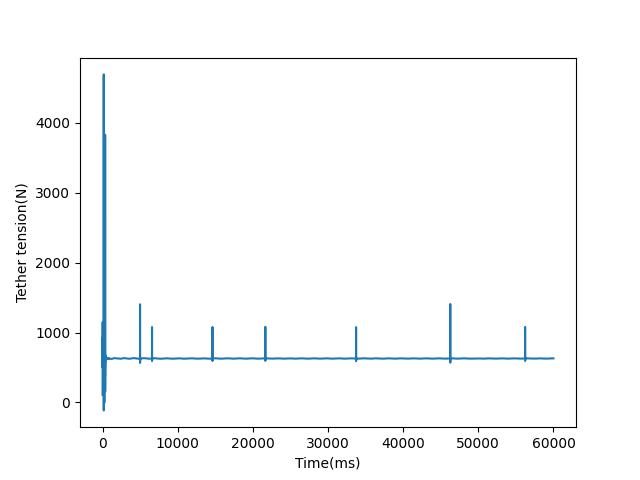
\includegraphics[width=0.9\textwidth]{tow0}
		\caption{\(v=0\)}
	\end{subfigure}
	\hfill
	\begin{subfigure}[b]{0.7\textwidth}
		\centering
		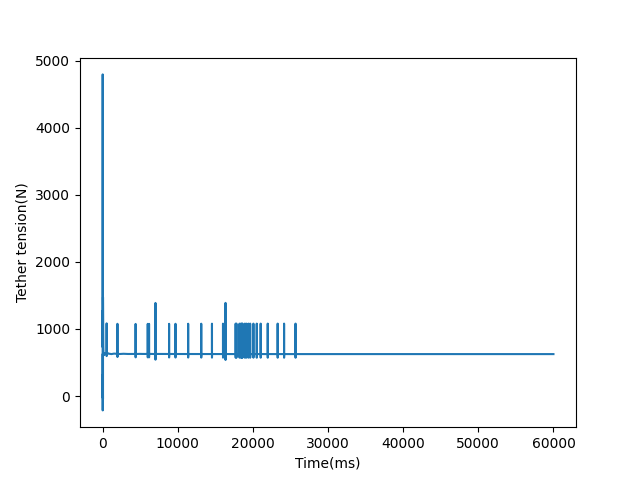
\includegraphics[width=0.9\textwidth]{tow1}
		\caption{\(v=1\frac{m}{s}\)}
	\end{subfigure}
	\hfill
	\begin{subfigure}[b]{0.7\textwidth}
		\centering
		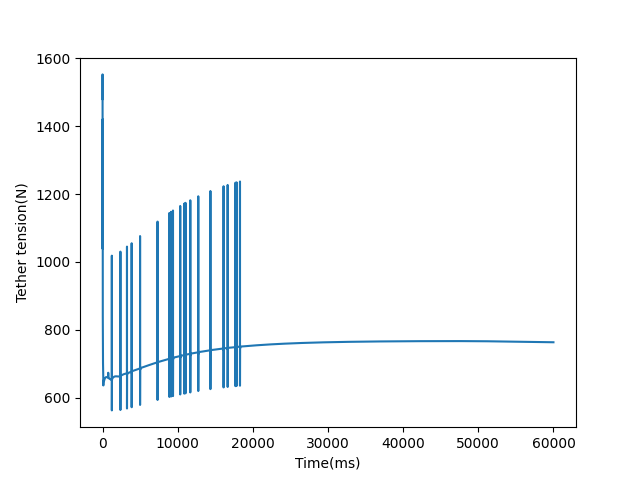
\includegraphics[width=0.9\textwidth]{tow2}
		\caption{\(v=2\frac{m}{s}\)}
	\end{subfigure}
\end{figure}

\begin{figure}\ContinuedFloat
	\centering
	\begin{subfigure}[b]{0.7\textwidth}
		\centering
		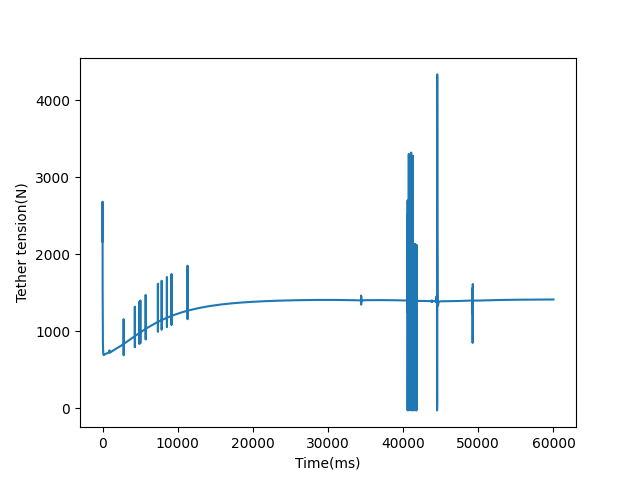
\includegraphics[width=0.9\textwidth]{tow3}
		\caption{\(v=3\frac{m}{s}\)}
	\end{subfigure}
	\hfill
	\begin{subfigure}[b]{0.7\textwidth}
		\centering
		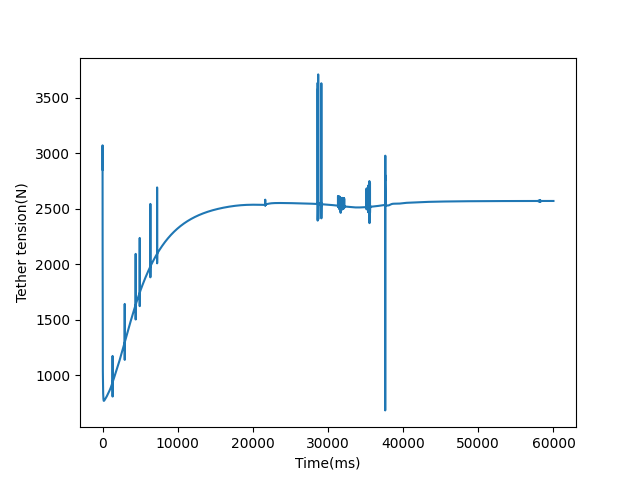
\includegraphics[width=0.9\textwidth]{tow4}
		\caption{\(v=4\frac{m}{s}\)}
	\end{subfigure}
	\hfill
	\begin{subfigure}[b]{0.7\textwidth}
		\centering
		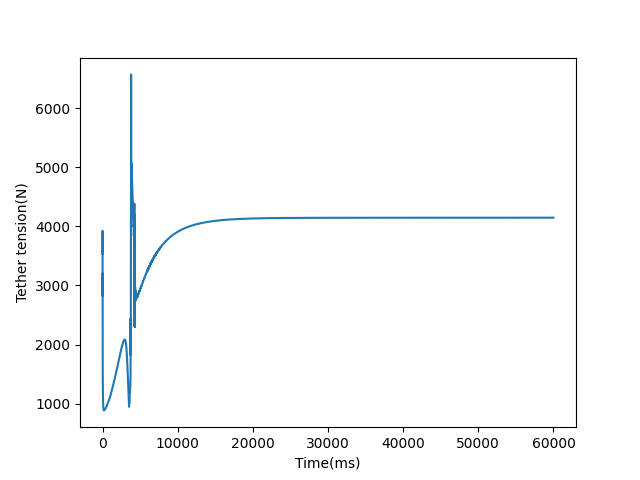
\includegraphics[width=0.9\textwidth]{tow5}
		\caption{\(v=5\frac{m}{s}\)}
	\end{subfigure}
	\caption{Graphs of tension in the towing tether at different towing speeds. The graphs are spiky at points, this is further discussed in \cref{sec:spiky}}
	\label{fig:tensions}
\end{figure}

\section{Control system results}
The control system has been implemented as a simple PD controller. The weights for the controller are set to 
\begin{align*}
k_p &= m_{\text{surf}}\omega^2 \\
k_d &= 2m_{\text{surf}}\zeta\omega
\end{align*}
Where \(m_{\text{surf}}\) is the mass of the surface vessel, \(\omega\) is a damping frequency and \(\zeta\) is the damping ratio. Through experimentation, I found that \(\omega = 0.45\) and \(\zeta = 1.2\) gave good results for this vessel. 

The way the controller is implemented it is able to take in a list of several targets and will treat them as individual targets sequentially. Once the vessel has reached one within a given acceptable error (currently set to 0.1m), the next target in the list is selected and the vessel moves towards it. The target selection finds not only if the current step has achieved the goal but also checks the errors for the last 50 timesteps. This is done so that the vessel couldn't hypothetically run straight through the waypoints, and instead has to actually come to a stop (or close to it) at the target positions. The number 50 was chosen arbitrarily. While there is a simple heading controller implemented, heading error is not taken into account with whether the vessel has reached the target or not. 

One simulation with the control system was done with 4 waypoints. The vessel moved from the starting point at (0,0) to (10,15) to (50, -30) to (-20,10) and back to (0,0). The route has been illustrated in \cref{fig:route}. These points were chosen arbitrarily and were chosen because they are a fair distance away from each other. In total, the theoretical shortest distance to travel would be roughly 180m. The time taken for the simulated vessel to move was 208s, or approximately 3.5 minutes. The total error can be seen in \cref{fig:error}. 

\begin{figure}
	\centering
	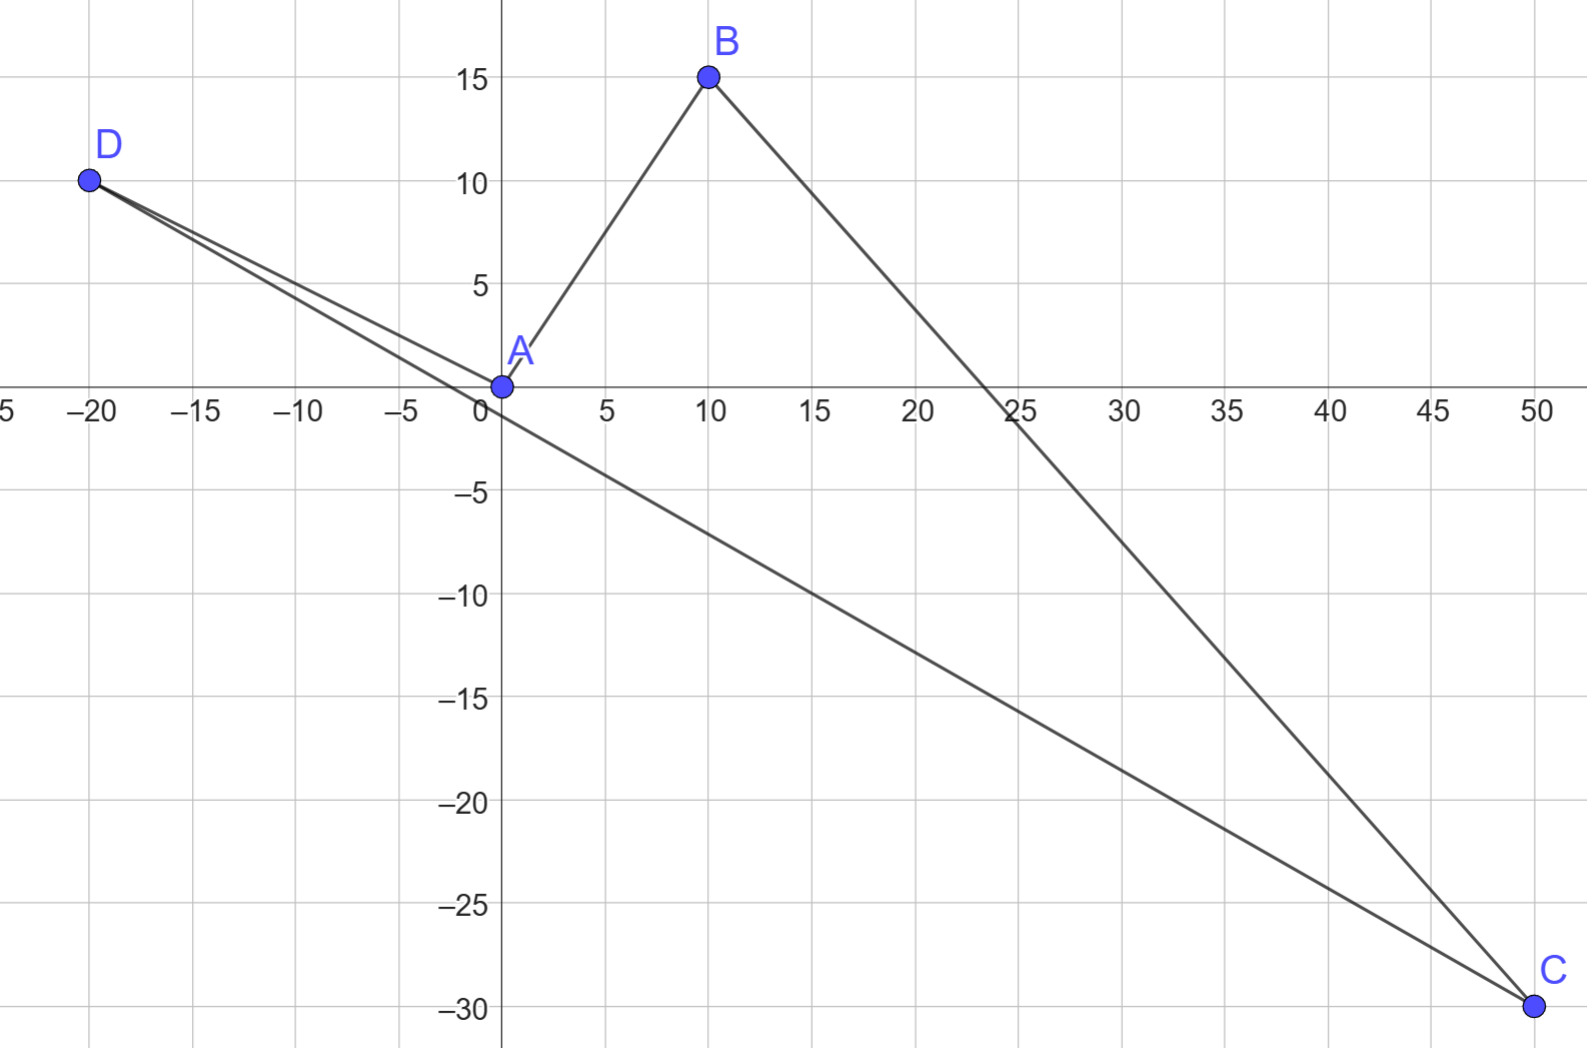
\includegraphics[width=0.8\textwidth]{route}
	\caption{The route the vessel was controlled through. Starting at A it moved through B, C and D before going back to A. Returning to start is not a requirement of the controller but was chosen as a waypoint}
	\label{fig:route}
\end{figure}

\begin{figure}
	\centering
	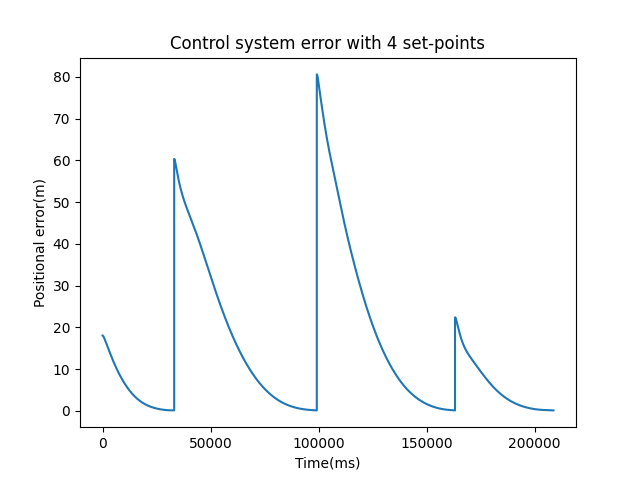
\includegraphics[width=0.8\textwidth]{control-error}
	\caption{Total error for the vessel between the four waypoints}
	\label{fig:error}
\end{figure}

%\cleardoublepage


\chapter{Discussion}
\section{Use as a rapid prototyping tool}
The solution shows a lot of promise as a rapid prototyping tool. As it stands at time of writing, the solution is fairly easy to configure for different initial conditions, depths of water/length of cable. Configuring the seastate is somewhat more complex as it's necessary to describe an elevation function for the sea surface. Sea currents also are not yet implemented, although AGX does allow for currents using the \texttt{WaterFlowGenerator} interface. 


\subsection{Ease of use}

\section{Future applicability}
The goal of this project has been to find 
\subsection{IRL testing proposal}
Master thesis etc.
%\cleardoublepage


\chapter{Conclusions}
The stated goal of the project has been to make a simulation of the Plan Sea project's proposed implementation. The project consists of a small surface vessel and a non-buoyant remotely operated vehicle attached to each other by a lifting wire. The simulation has been made to allow for control system design, as well as to act as an engineering tool for this specific project, allowing different sizes and types of wires to be used, allowing for changing sea-state and currents, or the type and size of vessels. 

In this report I've documented why the simulation would be a helpful tool for prototyping. I've also described some of the reasons why I believe simulation is more helpful for this case than finding analytical solutions to the problems posed by the project. 

I have created the simulation and run some validation tests on it to see whether it acts close to as should be expected from a realistic simulation. I have also created a simple PD-control system which is able to position the surface vessel at desired points in the world-space. The results found show that the simulation is likely more accurate than the simple analytical methods used to estimate the forces that would act on the system. 

I have proposed a list of topics for future iterations of the simulator, as well as stating my goal of continuing work on the simulator to use it for further development of the Plan Sea project. 

In all, I would count this project a success. The simulator has been created and validated, and is now ready for further processing and use in the Plan Sea project.


%\cleardoublepage

\newpage
\addcontentsline{toc}{chapter}{\protect\numberline{}Bibliography}
\printbibliography %you may change the title in the toc here if you want
%\cleardoublepage


%\chapter*{\LARGE \textbf{Appendices}}
\fancyhf{} %clear the header, it should be empty for the appendices
\renewcommand{\headrulewidth}{0pt} %no rule
\fancyfoot[C]{\thepage} %set the page numbers in the center of the footer instead 

%it is possible to set a different page numbering style for the appendix, but I personally just continued with the same page numbering as the main content as I find that more tidy
%\pagenumbering{roman}
%\setcounter{page}{1}%
%\addcontentsline{toc}{chapter}{\protect\numberline{}Appendices:}
%\appendix
%

\chapter*{A - Github repository}
\addcontentsline{toc}{chapter}{\protect\numberline{}A - Github repository} 

All code and latex-files used in this document are included in the Github repository linked below. Further explanations are given in the readme-file. 


\subsection*{Github repository link}
\begin{itemize}
    \item \url{https://github.com/ninasalvesen/thesis_latex_template}
\end{itemize}


%%%%%%%%%%%%%%%%%%%%%%%%%%%%%%%%%%%%%%%%%%%%%%%%%%%%%%%%


\chapter*{B - Sidenote statistics}
\addcontentsline{toc}{chapter}{\protect\numberline{}B - Sidenote statistics} 

%For included tables and figures renew the numbering such that they are numbered by the appendix they are attached to and not to the conclusion chapter
\renewcommand{\thefigure}{B.\arabic{figure}}
\setcounter{figure}{0}
\renewcommand{\thetable}{B.\arabic{table}}
\setcounter{table}{0}


\section*{\large{B1 - Some random table}}
\vspace*{1cm}

Remember to only include one thing per page in the appendices.

\begin{table}[ht!]
\centering
    \begin{tabular}{ m{4cm} m{2.5cm} m{2.5cm} m{2.5cm} } 
    \toprule
    \toprule
    \textbf{Statistic} & \textbf{One} & \textbf{Two}  \\
    \midrule
    Count   & 387317    & 283960    \\[1.3ex]
    Mean    & 130.66    & 134.18    \\[1.3ex]
    Std     & 248.09    & 230.32    \\[1.3ex]
    Q1      & 31.00     & 21.00     \\[1.3ex]
    Median  & 67.00     & 63.00     \\[1.3ex]
    Q3      & 142.00    & 159.00    \\[1.3ex]
    Min     & 0.00      & 0.00      \\[1.3ex]
    Max     & 14519.00  & 14253.00  \\[1.3ex]
    \bottomrule
    \bottomrule
    \end{tabular}
\caption[Statistics on something]{Table of statistics on some sidenote data.}
\end{table}


% Page without title but section title:
\newpage
\section*{\large{B2 - Some other random table}}
\vspace*{1cm}

\begin{table}[ht!]
\centering
    \begin{tabular}{ m{4cm} m{2.5cm} m{2.5cm} m{2.5cm} } 
    \toprule
    \toprule
    \textbf{Statistic} & \textbf{Three} & \textbf{Four}  \\
    \midrule
    Count   & 387317    & 283960    \\[1.3ex]
    Mean    & 130.66    & 134.18    \\[1.3ex]
    Std     & 248.09    & 230.32    \\[1.3ex]
    Q1      & 31.00     & 21.00     \\[1.3ex]
    Median  & 67.00     & 63.00     \\[1.3ex]
    Q3      & 142.00    & 159.00    \\[1.3ex]
    Min     & 0.00      & 0.00      \\[1.3ex]
    Max     & 14519.00  & 14253.00  \\[1.3ex]
    \bottomrule
    \bottomrule
    \end{tabular}
\caption[Statistics on something else]{Table of statistics on some other sidenote data.}
\end{table}



\newpage
\section*{\large{B3 - Some random figure}}
\vspace*{1cm}

\begin{figure}[H]
  \centering
  \subfloat[Data set sizes for data X.]
  {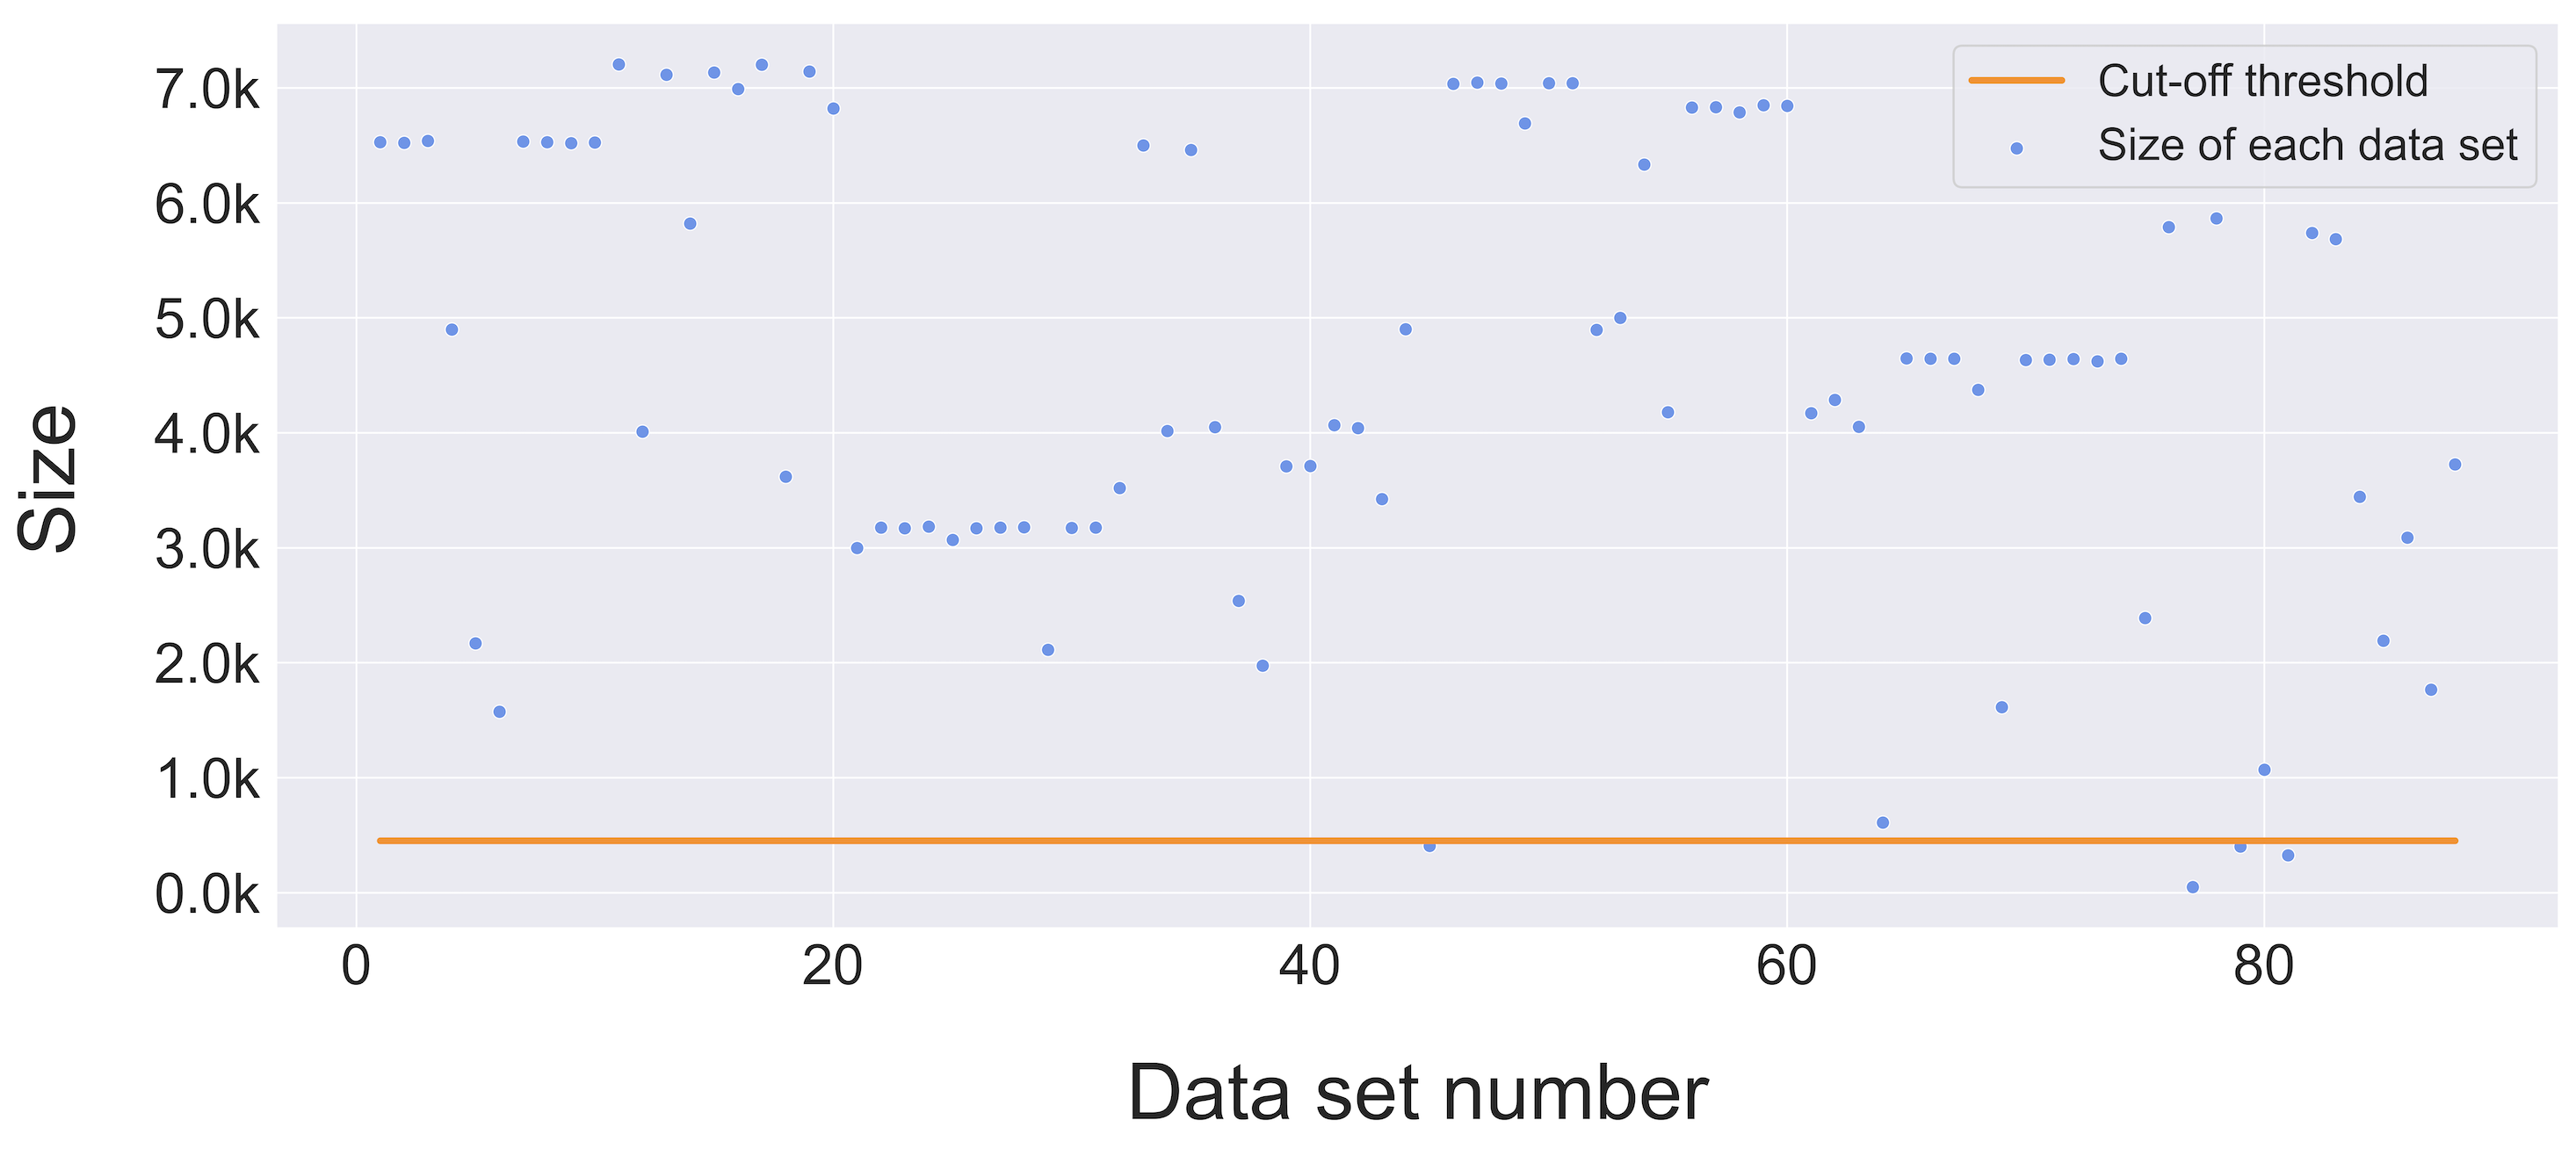
\includegraphics[width=1\textwidth]{Figures/dataset_X.png}}
  \hfill
  \subfloat[Data set sizes for data Y.]
  {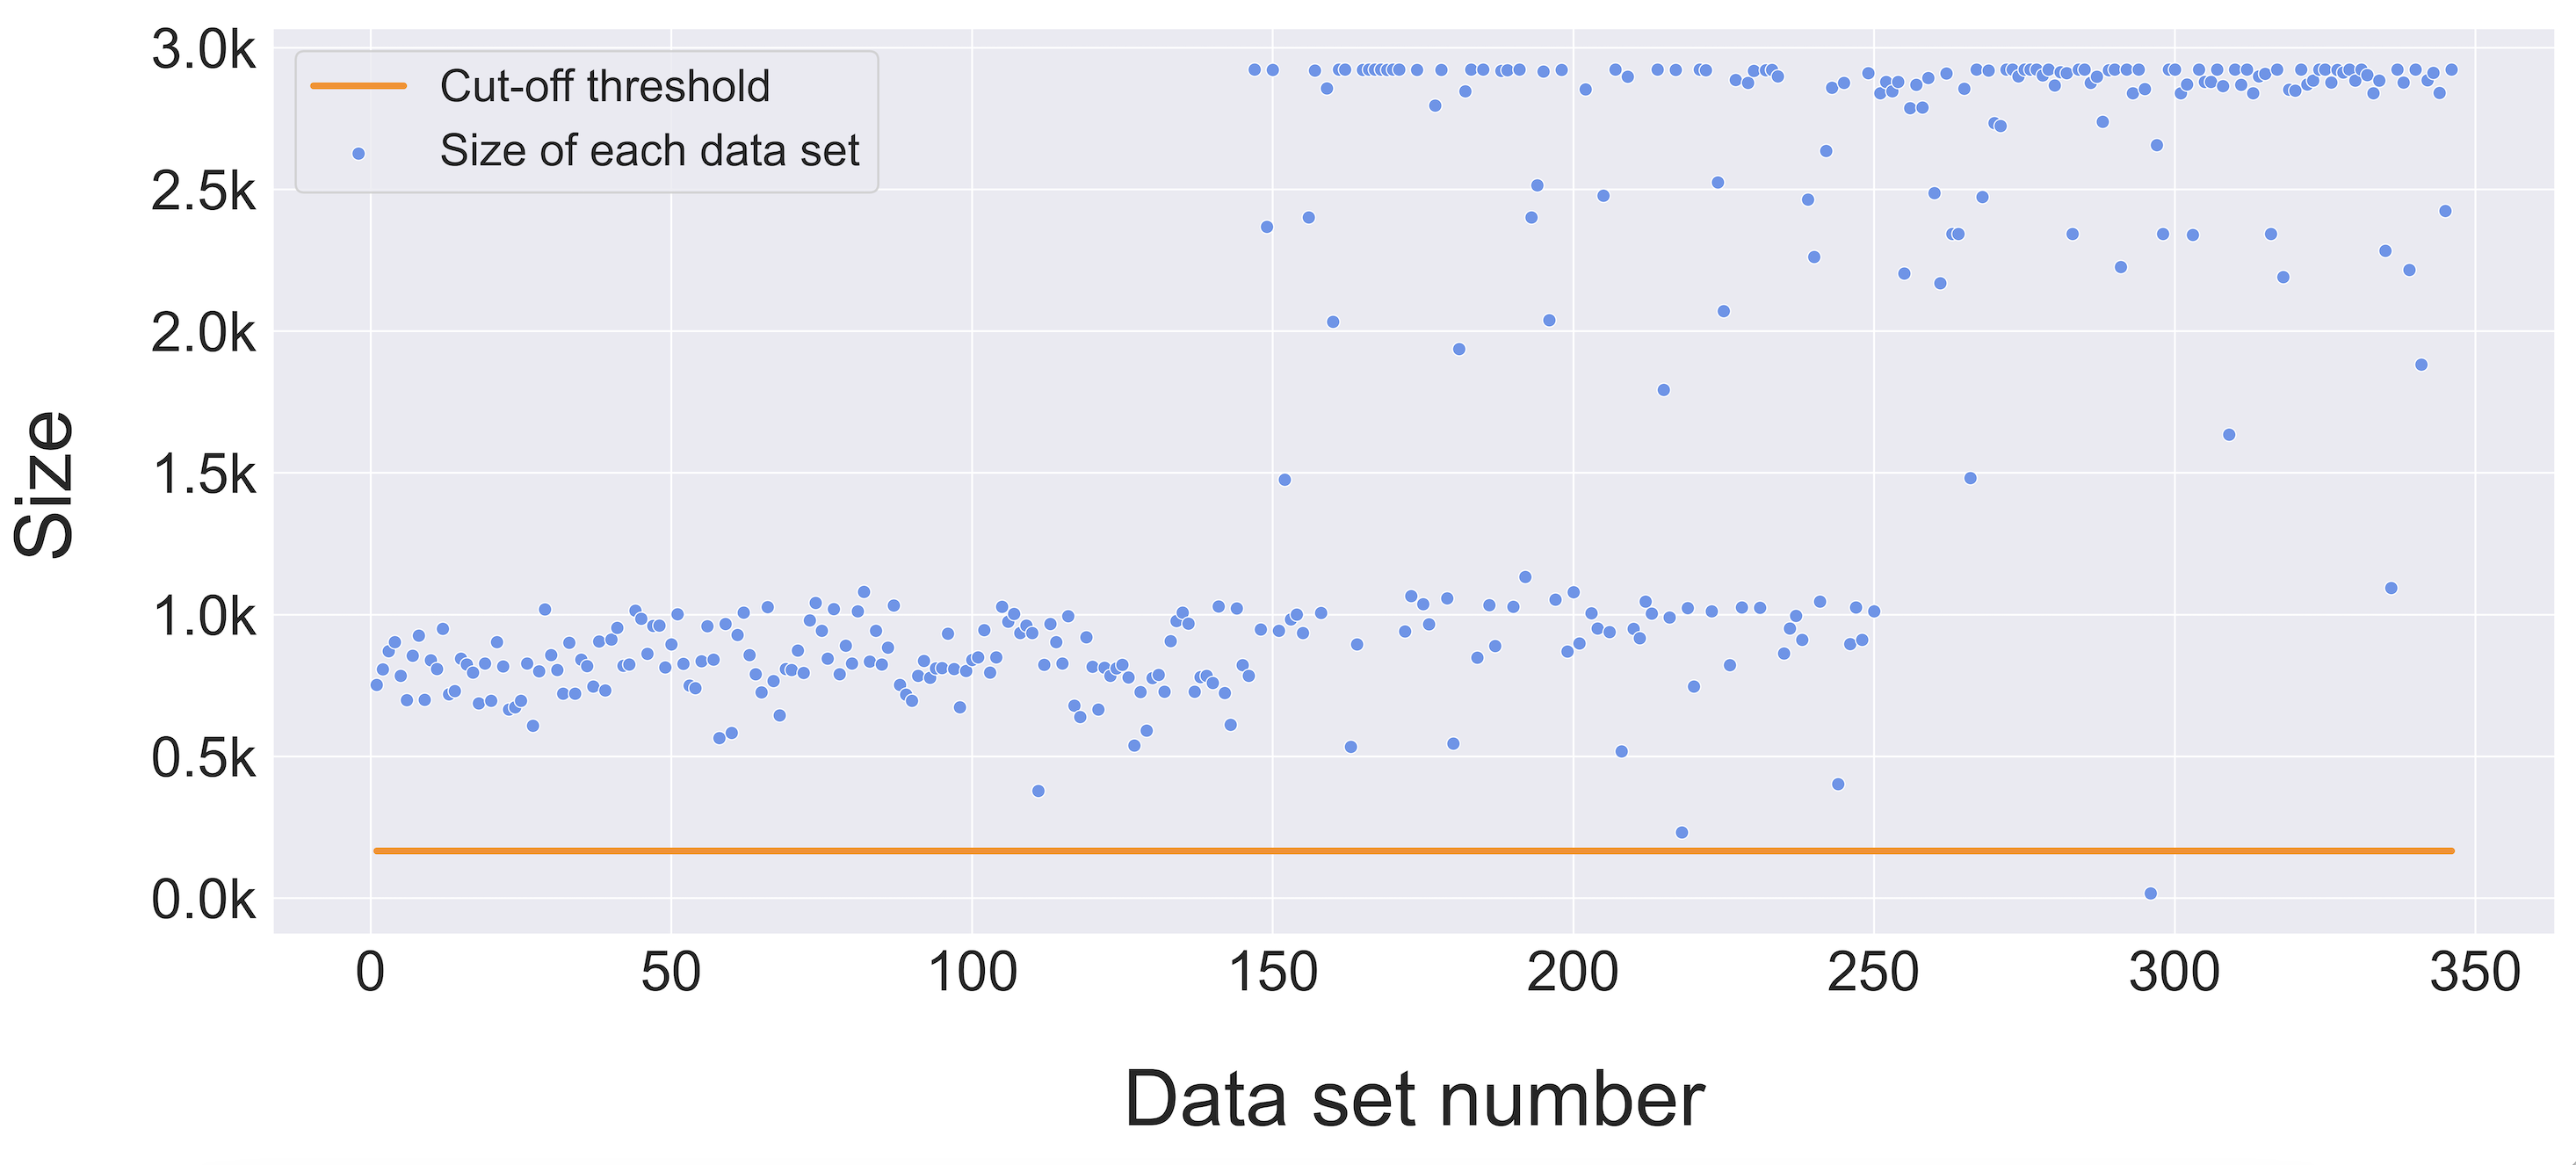
\includegraphics[width=1\textwidth]{Figures/dataset_Y.png}}
  \caption[Data set sizes]{The figures show the data set sizes of X and Y and the proposed cut-off threshold at 10 $\%$ of the mean set size.}
\end{figure}



%%%%%%%%%%%%%%%%%%%%%%%%%%%%%%%%%%%%%%%%%%%%%%%%%%%%%%%%


\end{document}
